\documentclass[main.tex]{subfiles}

\begin{document}

\hrulefill

Jan 30, 2017

\vspace{3mm}

What else do we need to know about $f(u)$ to be able to tell what kind of equilibra it is?

\begin{figure*}
\begin{multicols}{2}
    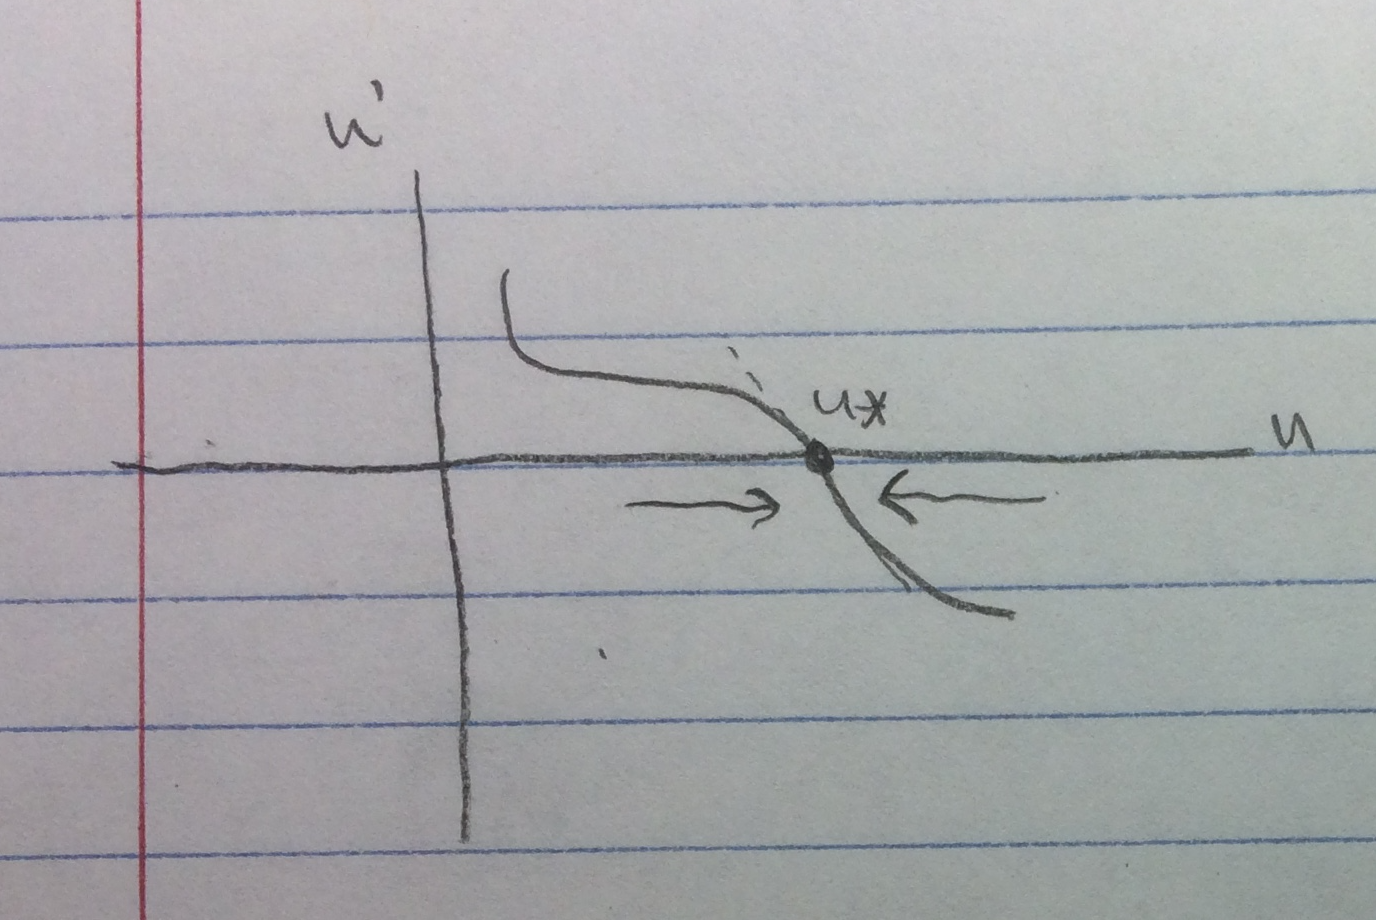
\includegraphics[width=\linewidth]{stable-intersect}\par 
    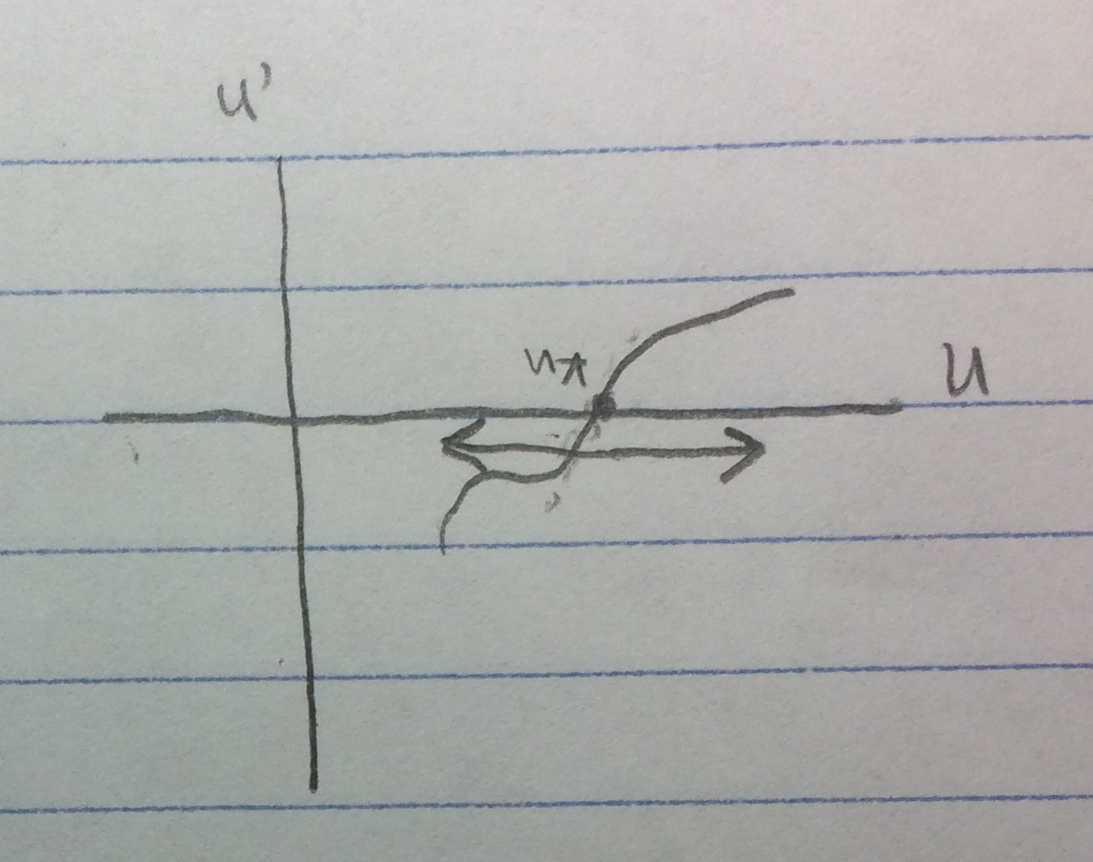
\includegraphics[width=\linewidth]{unstable-intersect}\par 
\end{multicols}
\begin{multicols}{2}
    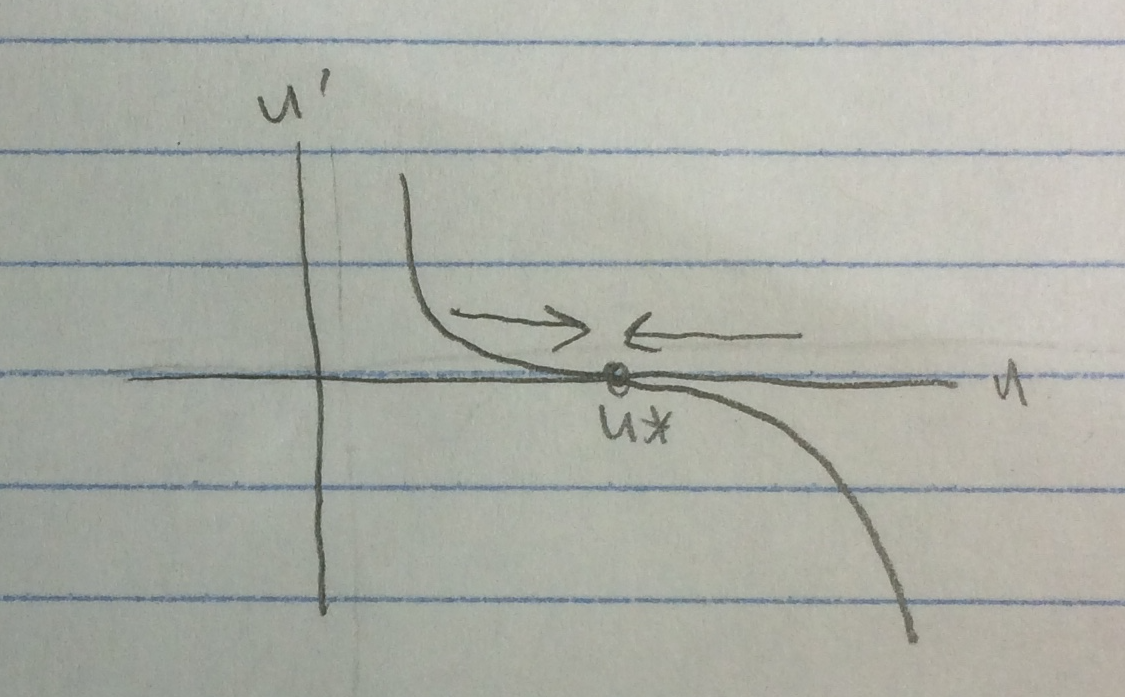
\includegraphics[width=\linewidth]{stable-tangent}\par
    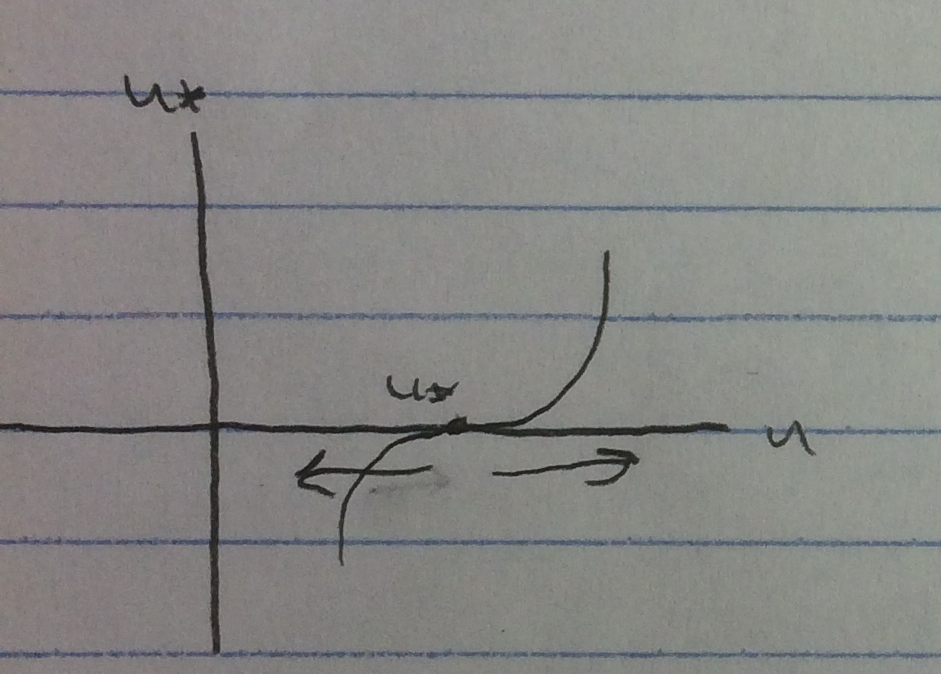
\includegraphics[width=\linewidth]{unstable-tangent}\par
\end{multicols}
\caption{Left panels: stable equilibria; Right panels: unstable equilibria}
\end{figure*}
\begin{figure*}
\begin{multicols}{2}
    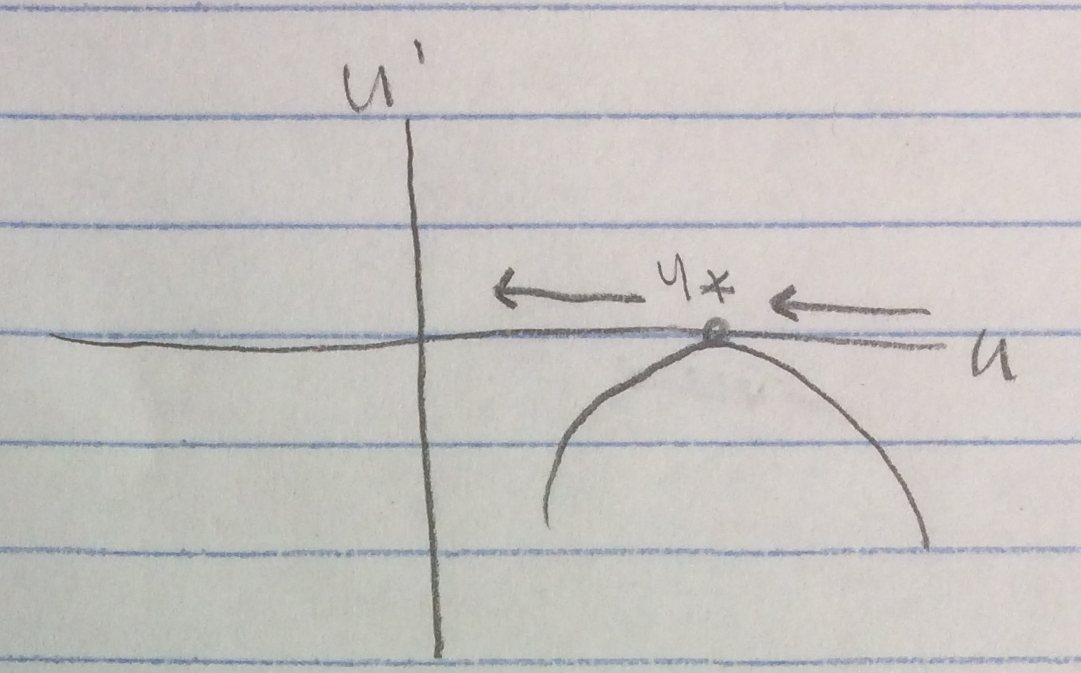
\includegraphics[width=\linewidth]{semistable-left}\par
    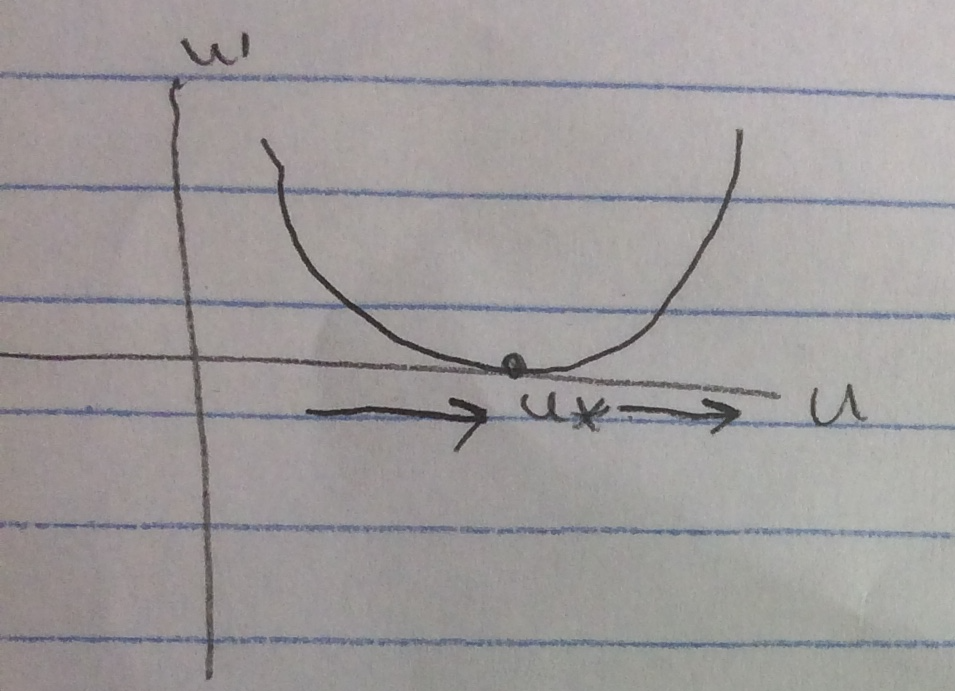
\includegraphics[width=\linewidth]{semistable-right}\par
\end{multicols}
\begin{multicols}{2}
    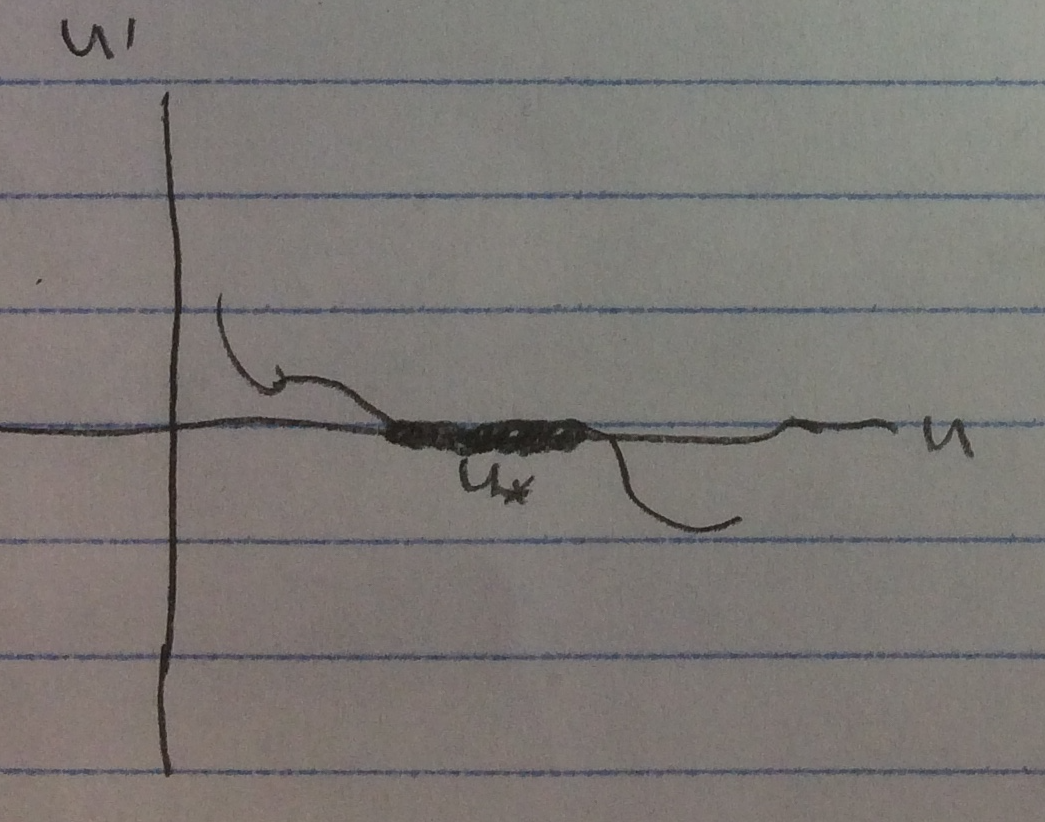
\includegraphics[width=\linewidth]{many-equilibria}\par
    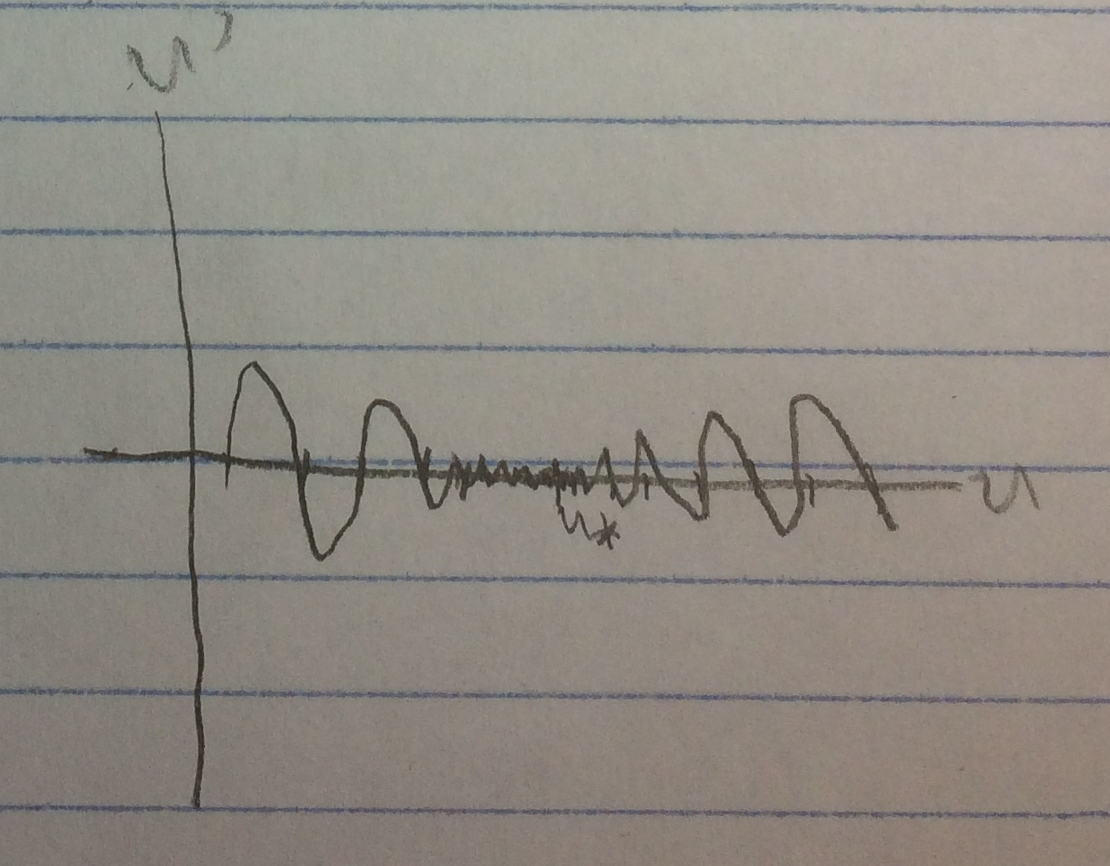
\includegraphics[width=\linewidth]{infinite-equilibria}\par
\end{multicols}
\caption{Upper panels: semistable equilibria.
Bottom left: Many equilibria, need to examine the graph.
Bottom right: More and more equilibria approaching $u_\star$}
\end{figure*}

%
%\begin{itemize}
%    \item If $f'(u_\star) > 0$, then $u_\star$ is unstable
%
%    Reason: On the left, you move away (slope is negative). On the right, you move away.
%    \item If $f'(u_\star) < 0$, then $u_\star$ is stable
%
%    Reason: On the left, you move towards (slope is positive). On the right, you move towards.
%
%    \item Missing case: $u_\star$ is an equilibrium but $f'(u_\star)$ = 0
%    \begin{itemize}
%        \item
%
%        \begin{figure}[ht]
%            \centering
%            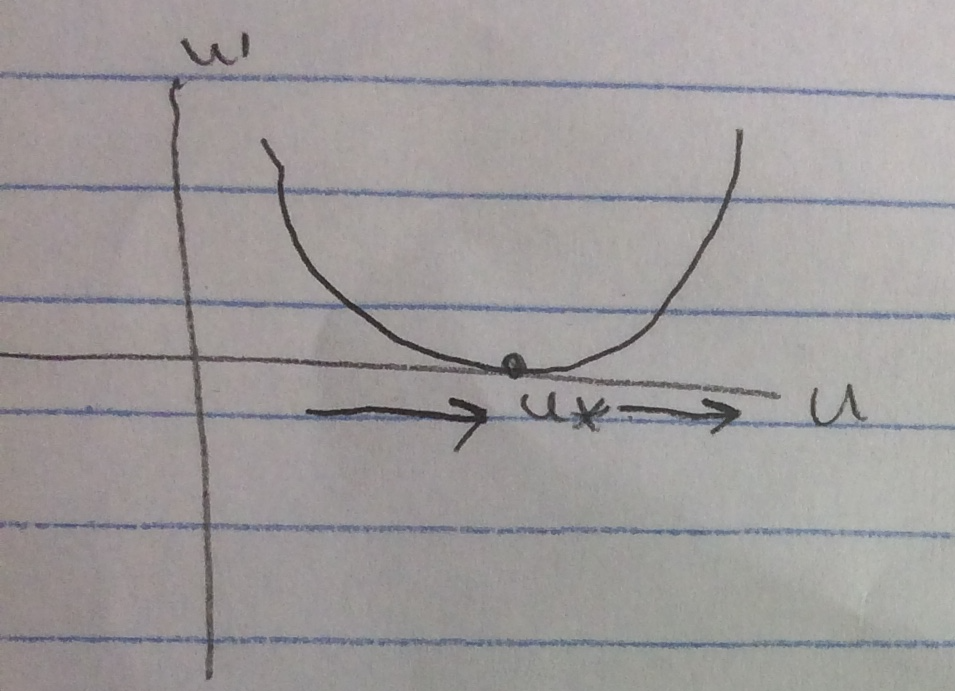
\includegraphics[width=0.5\textwidth]{semistable-right}
%            \caption{A system of masses connected with springs, separated by distance $h$ and with mass $m$.}
%            \label{fig:discrete-mass-spring-wave}
%        \end{figure}
%
%        \item Stable (TODO: INSERT FIGURE)
%        \item Unstable (TODO: INSERT FIGURE)
%        \item Many close equilibria (TODO: INSERT FIGURE)
%        \item Many close equilibria (TODO: INSERT FIGURE)
%    \end{itemize}
%\end{itemize}

\textbf{Revisiting bead on hoop}

$$\begin{cases}
    \dot{\phi} = a\sin{\phi}(\mu\cos{\phi-1}) \\
    a\textrm{, }\mu > 0 \\
    \mu = \frac{r\omega^2}{g} \textrm{\textasciitilde} \omega^2
\end{cases}$$

Find equilibra:
$$a\sin{\phi}(\mu\cos{\phi-1}) = 0$$
$$\sin{\phi} = 0 \implies \phi_\star = \{0, \pi\}$$
Stability of these equilibra:
$$f'(\phi) = \left(a\cos{\phi}(\mu\cos{\phi} - 1) - a\mu\sin^2{\phi}\right)$$
\begin{itemize}
    \item $f'(0) = a(\mu - 1)$
    \begin{itemize}
        \item When $\mu > 1$, $f'(0) > 0$ therefore unstable
        \item When $\mu < 1$, $f'(0) < 0$ therefore stable
        \item When $\mu = 1$, $f'(0) = 0$ so gotta look at graph.
    \end{itemize}
    \item $f'(\pi) = a(\mu + 1)$ is always positive, so $f(\pi)$ is unstable.
\end{itemize}

This all implies that when the hoop is rotated slowly, the equilibrium at $\phi = 0$ is stable. When it's rotated quickly, the equilibria is unstable.

Now to examine the other term $\mu\cos{\phi} - 1$.
$\mu\cos{\phi} - 1\implies \cos{\phi} = 1/\mu$

Diagrams:

\begin{figure*}
\begin{multicols}{2}
    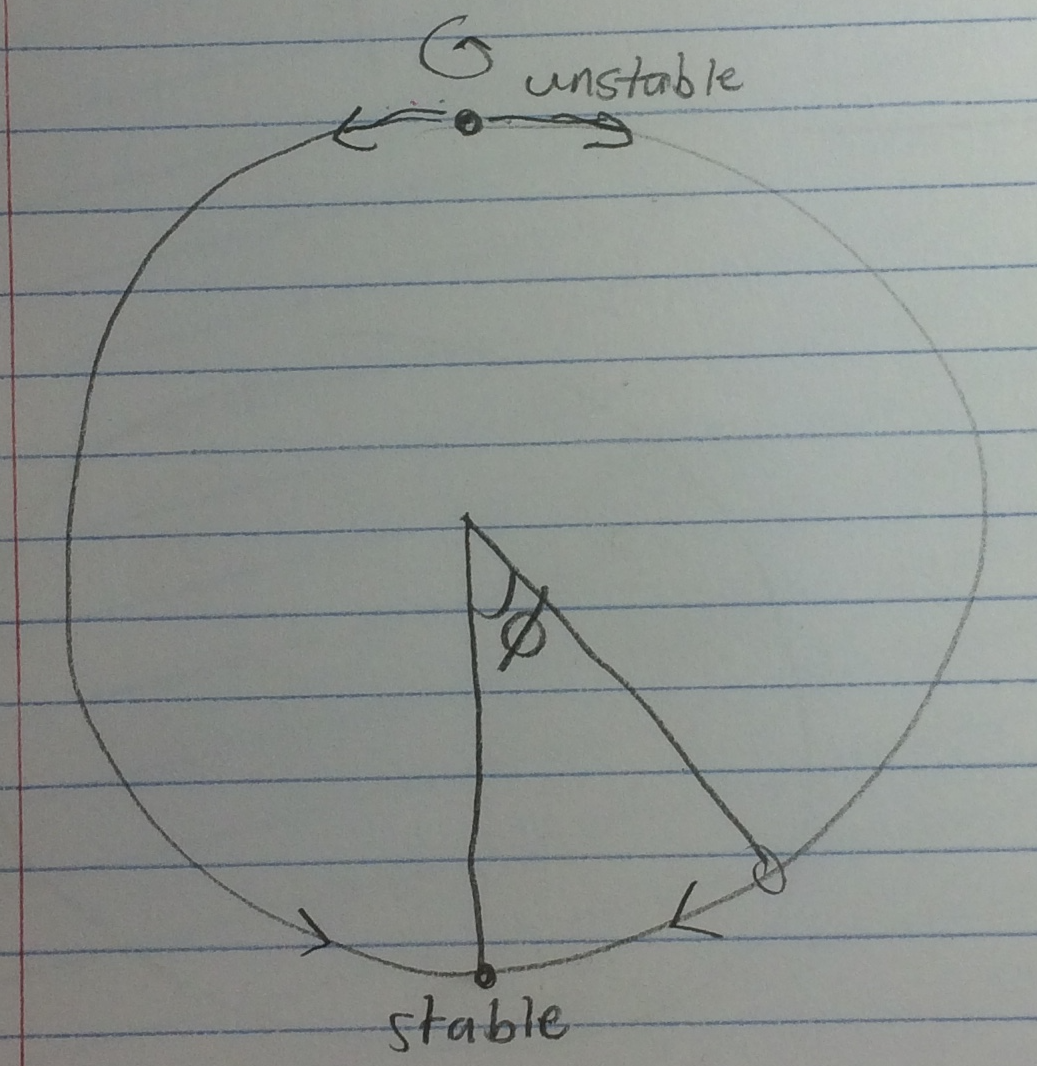
\includegraphics[width=\linewidth]{hoop-bead-low-omega}\par
    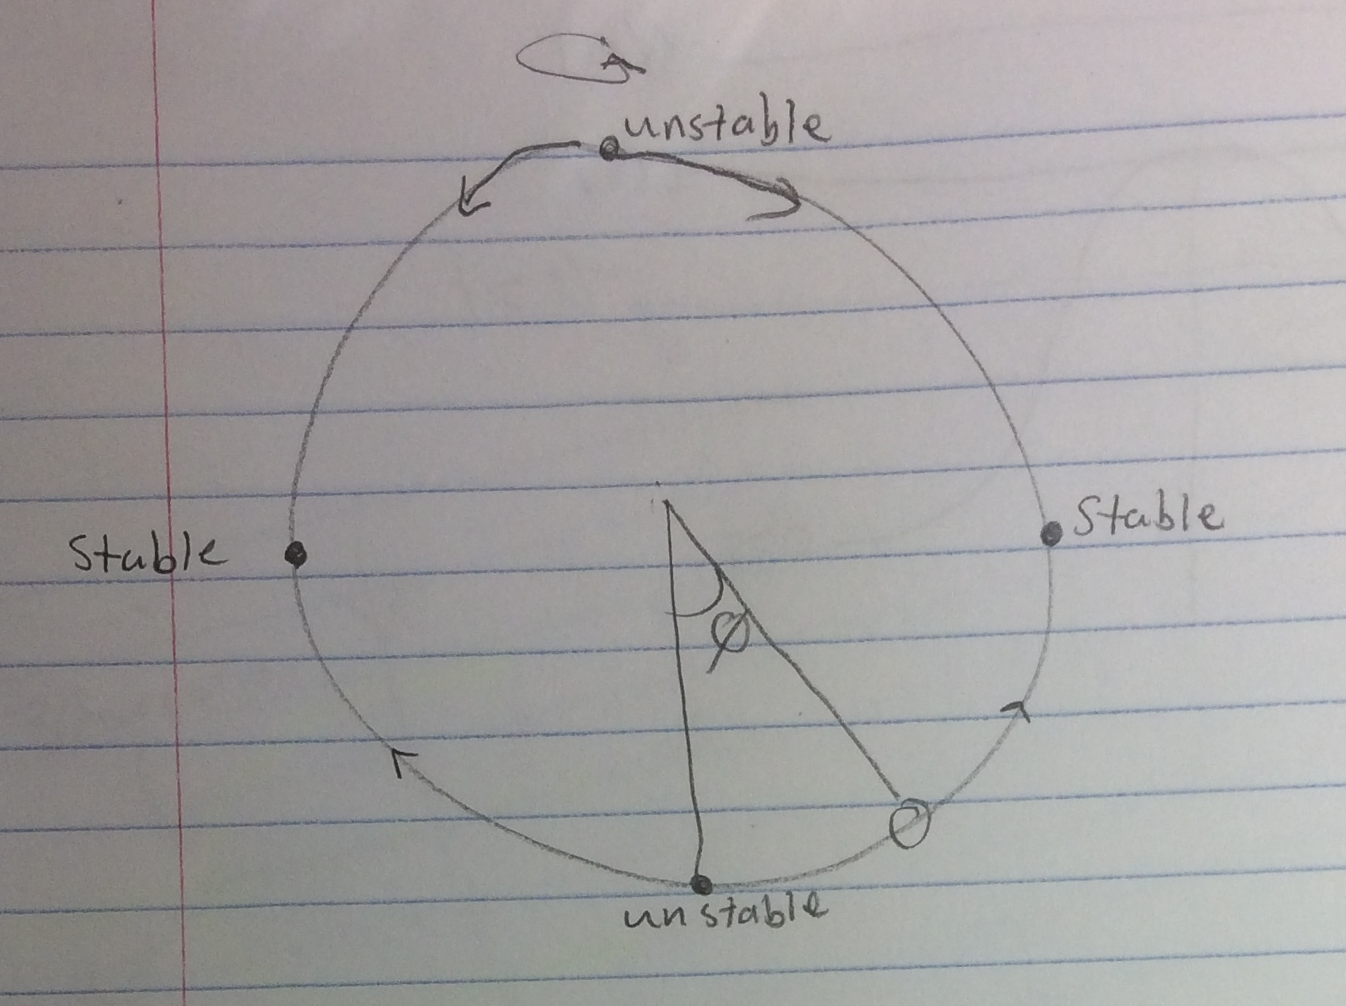
\includegraphics[width=\linewidth]{hoop-bead-high-omega}\par
\end{multicols}
\caption{Left: The hoop is rotated slowly, so the bead will fall to the bottom stable equilibrium.
         Right: The hoop is rotated very fast. As $\omega$ goes to infinity, the $\phi$ approaches $\pi/2$.}
\end{figure*}

Bifurcation diagram:
\begin{figure}[ht]
        \centering
        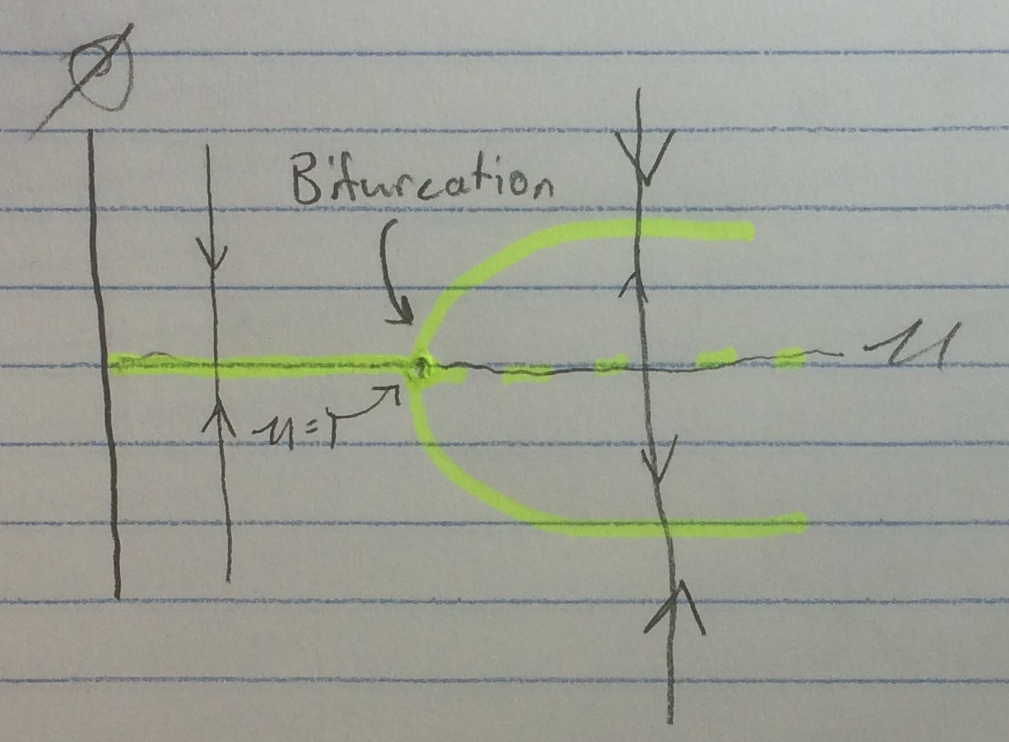
\includegraphics[width=0.5\textwidth]{hoop-bead-phi-of-miu}
        \caption{The bifurcation diagram for this system}
        \label{fig:hoop-bead-bifurcation}
\end{figure}
\end{document}
